\paragraph{}{
	Le décodeur d'instructions permet de déterminer quel opération va effectuer
	le processeur pour le cycle à venir. C'est lui qui lit les opcodes déterminés
	précédemment.
}
	\subparagraph{Gestion des sauts}{
		Lorsque le décodeur de sauts lis une instruction de type \textit{b},
		il se contente d'appeler l'Unité Arithmétique et Logique pour faire
		une soustraction. Il arme également la sortie \textit{isJMP}.
	}

\begin{figure}
	\centering
	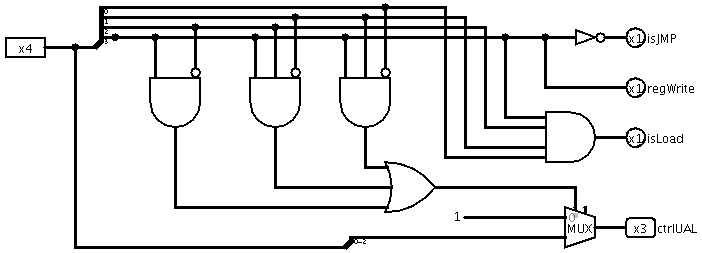
\includegraphics[scale=0.4,origin=c]{circuits/deco_instru.png}
	\caption{
		\label{decod_inst_circ}
		Sch\'{e}ma \'{e}lectronique pour le d\'{e}codeur d'instructions
		}
\end{figure}

\paragraph{}{
	Le schéma électronique du décodeur d'instructions est présenté à la figure
	\ref{decod_inst_circ}. La partie qui décode le signal \textit{ctrlUAL} 
	correspond au tableau de \textsc{Karnaugh} de la figure 
	\ref{decod_ctrlual_karnaugh} duquel on extrait l'équation \ref{ual_eq}.
}


\begin{figure}
	\begin{center}
	\centering
	\begin{tabular}{|c|c|c|c|c|}
		\hline
		\backslashbox{$b_{3}b_{2}$}{$b_{1}b_{0}$} & $00$ & $01$ & $11$ & $10$ \\ 
		\hline 
		$00$ & $0$ & $0$ & $0$ & $0$ \\ 
		\hline 
		$01$ & $0$ & $0$ & $0$ & $0$ \\ 
		\hline 
		$11$ & $1$ & $1$ & $0$ & $1$ \\ 
		\hline 
		$10$ & $1$ & $1$ & $1$ & $1$ \\ 
		\hline 
	\end{tabular} 
	\end{center}
	\caption{
		\label{decod_ctrlual_karnaugh}
		Tableau de \textsc{Karnaugh} pour le décodage d'instructions.
	}
\end{figure}

	\begin{equation}
		ctrlUAL = b_{3} . \neg b_{2} + b_{3} . b_{2} \neg b_{1}  + b_{3} . b_{1} \neg b_{0}
		\label{ual_eq}
	\end{equation}

\paragraph{}{
	Cette équation nous permet alors de réaliser le circuit électronique 
	décodant \textit{ctrlAUL}. Les variables $b_{3}$, $b_{2}$, $b_{1}$ 
	et $b_{0}$ correspondent aux bits de l'opcode.
}